\documentclass[tikz,border=4pt]{standalone}
\usepackage{pgfplots}
\pgfplotsset{compat=1.18}
\definecolor{accB}{HTML}{1769AA}
\definecolor{accO}{HTML}{C85A00}
\definecolor{ink}{HTML}{18212B}
\definecolor{slate}{HTML}{66727D}
\definecolor{gridg}{HTML}{E4E7EA}
% note (luojiaxuan): 预算趋势折线(全量 117):蓝=Recent-B,橙=CausalCache;
% B=0 两臂同一点(结构性等价),线型分离 + B=4 主设置点直标。
\begin{document}
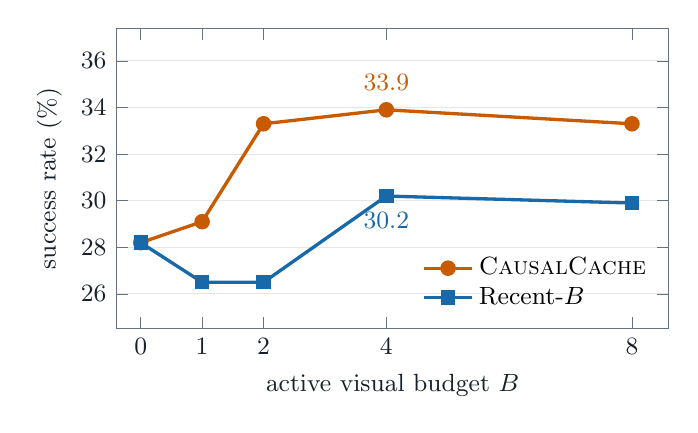
\begin{tikzpicture}
\begin{axis}[
  width=8.6cm, height=5.4cm,
  xlabel={active visual budget $B$}, ylabel={success rate (\%)},
  xmin=-0.4, xmax=8.6, ymin=24.5, ymax=37.4,
  xtick={0,1,2,4,8}, ytick={26,28,30,32,34,36},
  axis line style={slate}, tick style={slate},
  ticklabel style={font=\small, color=ink},
  label style={font=\small, color=ink},
  ymajorgrids, grid style={gridg},
  legend style={at={(0.985,0.03)}, anchor=south east, font=\small,
    draw=none, fill=none, row sep=-1pt},
  legend cell align=left,
]
\addplot[accO, very thick, mark=*, mark size=2.2pt]
  coordinates {(0,28.2) (1,29.1) (2,33.3) (4,33.9) (8,33.3)};
\addlegendentry{\textsc{CausalCache}}
\addplot[accB, very thick, mark=square*, mark size=2.0pt]
  coordinates {(0,28.2) (1,26.5) (2,26.5) (4,30.2) (8,29.9)};
\addlegendentry{Recent-$B$}
% B=4 主设置直标
\node[font=\small, text=accO, anchor=south] at (axis cs:4,34.3) {33.9};
\node[font=\small, text=accB, anchor=north] at (axis cs:4,29.9) {30.2};
\end{axis}
\end{tikzpicture}
\end{document}
